%----------------------------------------------------------------------------------------
%	HOMEWORK ASSIGNMENT EE5251
%----------------------------------------------------------------------------------------

%----------------------------------------------------------------------------------------
%	PROLOUGE 
%----------------------------------------------------------------------------------------
\documentclass[a4paper, 11pt]{article}
\usepackage[scale=0.85]{geometry} 		% Reduce document margins
\usepackage{hyperref} 					% Required for hyperlinks i.e. e-mail %
\usepackage{titlesec} 					% Used to customize the \section command
\usepackage[T1]{fontenc}				% Used to have both Bold and Small caps in heading
\usepackage{amsmath}					% Used to write equations
\usepackage{amssymb}					% Used to write math symbols e.g. R = real number set
\usepackage{autobreak}
\usepackage{graphicx}					% Used to include images
\usepackage{tabularx} 					% For custom table %
\usepackage{mathtools}					% For define notation
\allowdisplaybreaks
%----------------------------------------------------------------------------------------
%	CUSTOM MACRO DEFINITION AND ENVIRONMENT MODIFICATION
%----------------------------------------------------------------------------------------
\titleformat{\section}{\bfseries\Large\scshape\filcenter}{}{0em}{}[{\titlerule[1pt]}] % Text formatting of sections
\titlespacing{\section}{0pt}{3pt}{3pt} % Spacing around sections
\pagestyle{empty} % Removes page numbering
\newcommand{\xVec}{\ensuremath{\boldsymbol{x}}}
\newcommand{\wVec}{\ensuremath{\boldsymbol{w}}}
\newcommand{\muVec}{\ensuremath{\boldsymbol{\mu}}}
\newcommand{\mVec}{\ensuremath{\boldsymbol{m}}}
\newcommand{\sVec}{\ensuremath{\boldsymbol{S}}}
\newcommand{\sigmaVec}{\ensuremath{\boldsymbol{\sigma}}}
\newcommand{\SigmaVec}{\ensuremath{\boldsymbol{\Sigma}}}
\DeclareMathOperator*{\minimize}{minimize}
%----------------------------------------------------------------------------------------
%	MAIN BODY
%----------------------------------------------------------------------------------------
\begin{document}
	%----------------------------------------------------------------------------------------
%	HEADER
%----------------------------------------------------------------------------------------
\section{HW 4}
\begin{tabularx}{\textwidth}{l}
	\hspace*{-0.8cm}\large\textsc{Arnab Dey}\\
	\hspace*{-0.8cm}Student ID: 5563169\\
	\hspace*{-0.8cm}Email: dey00011@umn.edu\\
\end{tabularx}
\bigskip
\par
    %----------------------------------------------------------------------------------------
%	SOLUTION 1
%----------------------------------------------------------------------------------------
\subsection*{Problem 1}
\paragraph{1.(a) Proof of $(AB)^T = B^TA^T$:}By definition, if $A \in \mathbb{R}^{m\times n}$ and $B \in \mathbb{R}^{n \times p}$, the $ij$ entry of $AB$,
\begin{align*}
	(AB)_{ij} = \sum_{k=1}^{n}a_{ik}b_{kj},
\end{align*}
where $a_{ik}$ is the $ik$ entry of $A$ and $b_{kj}$ is the $kj$ entry of $B$, $i \in \{1,2,\ldots,m\}, j \in \{1,2,\ldots,p\}$. Now, again by definition of transpose,
\begin{align*}
	(AB)^T_{ij} = (AB)_{ji} = \sum_{k=1}^{n} a_{jk}b_{ki}.
\end{align*}
Now,
\begin{align*}
	(B^TA^T)_{ij} &= \sum_{k=1}^{n}(B^T)_{ik}(A^T)_{kj}\\
	&= \sum_{k=1}^{n} b_{ki}a_{jk}\\
	&= \sum_{k=1}^{n}a_{jk}b_{ki} \\
	&= (AB)^T_{ij}.
\end{align*}
Therefore, $ij$ entry of $(B^TA^T)$ and $(AB)^T$ are equal for all $i \in \{1,2,\ldots,m\}, j \in \{1,2,\ldots,p\}$. Therefore,
\begin{align*}
	(AB)^T = B^TA^T.
\end{align*}
This completes the proof. $\square$
\paragraph{1.(b) Proof of $(AB)^{-1} = B^{-1}A^{-1}$:} Here, it is implied that the inverse of $AB \in \mathbb{R}^{n\times n}, A \in \mathbb{R}^{n \times p}$ and $B \in \mathbb{R}^{p \times n}$ exist. Therefore, let,
\begin{align*}
	&AB = C\\
	\implies& A^{-1}AB = A^{-1}C\\
	\implies& I_{p\times p}B = A^{-1}C\\
	\implies& B = A^{-1}C\\
	\implies& B^{-1}B = B^{-1}A^{-1}C\\
	\implies& I_{n \times n} = B^{-1}A^{-1}C\\
	\implies& I_{n \times n}C^{-1} = B^{-1}A^{-1}CC^{-1}\\
	\implies& C^{-1} = B^{-1}A^{-1}I_{n \times n}\\
	\implies& (AB)^{-1} = B^{-1}A^{-1}.
\end{align*}
This completes the proof. $\square$
\paragraph{1.(c) Proof of $\text{Tr}(AB) = \text{Tr}(BA)$:}By definition, if $A \in \mathbb{R}^{n\times p}$ and $B \in \mathbb{R}^{p \times n}$,
\begin{align*}
	\text{Tr}(AB) &= \sum_{k=1}^{n} (AB)_{kk}\\
	&= \sum_{k=1}^{n} \sum_{j=1}^{p}a_{kj}b_{jk}\\
	&= \sum_{j=1}^{p} \sum_{k=1}^{n}b_{jk}a_{kj}\\
	&= \sum_{j=1}^{p}(BA)_{jj}\\
	&= \text{Tr}(BA).
\end{align*}
This completes the proof. $\square$
%----------------------------------------------------------------------------------------
%	SOLUTION 2
%----------------------------------------------------------------------------------------
\subsection*{Problem 2}
Let, $A \in \mathbb{R}^{n \times p}$ and $B \in \mathbb{R}^{p \times n}$. We have to find $\frac{\partial}{\partial A}\text{Tr}(AB)$. Now,
\begin{align*}
	\frac{\partial}{\partial A} \text{Tr}(AB) &= \frac{\partial}{\partial A} \left[\sum_{k=1}^{n}\sum_{j=1}^{p}a_{kj}b_{jk}\right]\\
	&= \begin{bmatrix}\frac{\partial}{\partial a_{11}} \left[\sum_{k=1}^{n}\sum_{j=1}^{p}a_{kj}b_{jk}\right] & \ldots & \frac{\partial}{\partial a_{1p}} \left[\sum_{k=1}^{n}\sum_{j=1}^{p}a_{kj}b_{jk}\right]\\
	\vdots & \ldots & \vdots\\
	\frac{\partial}{\partial a_{n1}} \left[\sum_{k=1}^{n}\sum_{j=1}^{p}a_{kj}b_{jk}\right] & \ldots & \frac{\partial}{\partial a_{np}} \left[\sum_{k=1}^{n}\sum_{j=1}^{p}a_{kj}b_{jk}\right]\end{bmatrix}\\
	&= \begin{bmatrix}b_{11} & \ldots & b_{p1}\\
	\vdots & \ldots & \vdots\\
	b_{1n} & \ldots & b_{pn}\end{bmatrix}\\
	&= B^T.
\end{align*}
%----------------------------------------------------------------------------------------
%	SOLUTION 3
%----------------------------------------------------------------------------------------
\subsection*{Problem 3}
It is given that,
\begin{align*}
	\begin{bmatrix}A & A\\B & A\end{bmatrix}\begin{bmatrix}A\\C\end{bmatrix} = \begin{bmatrix}0\\I\end{bmatrix}.
\end{align*}
Therefore, by definition of block matrix multiplication,
\begin{align*}
	A^2 + AC &= 0\\
	BA + AC &= I.
\end{align*}
Solving the above two equations for $B$ and $C$, we get,
\begin{align*}
	C &= -A\\
	B &= A^{-1}+A.
\end{align*}
%----------------------------------------------------------------------------------------
%	SOLUTION 4
%----------------------------------------------------------------------------------------
\subsection*{Problem 4}
It is given that,
\begin{align*}
	P = \begin{bmatrix}1 & 2 & 2\\0 & 3 & 1\\0 & 1 & 2\end{bmatrix}.
\end{align*}
Let,
\begin{align*}
	A &= \begin{bmatrix}1 & 0 & 0\\0 & 2 & 0\\0 & 0 & 1\end{bmatrix}\\
	B &= \begin{bmatrix}2\\1\\1\end{bmatrix}\\
	C &= \begin{bmatrix}0 & 1 & 1\end{bmatrix}\\
	D &= 1.
\end{align*}
Therefore, it can be verified that,
\begin{align*}
	A+BD^{-1}C = P.
\end{align*}
Also,
\begin{align*}
	A^{-1} &= \begin{bmatrix}1 & 0 & 0\\0 & \frac{1}{2} & 0\\0 & 0 & 1\end{bmatrix}\\
	CA^{-1} &= \begin{bmatrix}0 & 1 & 1\end{bmatrix}\begin{bmatrix}1 & 0 & 0\\0 & \frac{1}{2} & 0\\0 & 0 & 1\end{bmatrix} = \begin{bmatrix}0 & \frac{1}{2} & 1\end{bmatrix}\\
	D+CA^{-1}B &= 1+\begin{bmatrix}0 & \frac{1}{2} & 1\end{bmatrix}\begin{bmatrix}2\\1\\1\end{bmatrix} = 1+\frac{1}{2}+1 = \frac{5}{2}.
\end{align*}
Therefore, using the matrix inversion lemma,
\begin{align*}
	P^{-1} &= (A+BD^{-1}C)^{-1}\\
	&= A^{-1}-A^{-1}B(D+CA^{-1}B)^{-1}CA^{-1}\\
	&= \begin{bmatrix}1 & 0 & 0\\0 & \frac{1}{2} & 0\\0 & 0 & 1\end{bmatrix}-\begin{bmatrix}1 & 0 & 0\\0 & \frac{1}{2} & 0\\0 & 0 & 1\end{bmatrix}\begin{bmatrix}2\\1\\1\end{bmatrix}\left(\frac{5}{2}\right)^{-1}\begin{bmatrix}0 & \frac{1}{2} & 1\end{bmatrix}\\
	&= \begin{bmatrix}1 & 0 & 0\\0 & \frac{1}{2} & 0\\0 & 0 & 1\end{bmatrix}-\begin{bmatrix}1 & 0 & 0\\0 & \frac{1}{2} & 0\\0 & 0 & 1\end{bmatrix}\begin{bmatrix}2\\1\\1\end{bmatrix}\begin{bmatrix}0 & \frac{1}{5} & \frac{2}{5}\end{bmatrix}\\
	&= \begin{bmatrix}1 & 0 & 0\\0 & \frac{1}{2} & 0\\0 & 0 & 1\end{bmatrix}-\begin{bmatrix}2\\\frac{1}{2}\\1\end{bmatrix}\begin{bmatrix}0 & \frac{1}{5} & \frac{2}{5}\end{bmatrix}\\
	&= \begin{bmatrix}1 & 0 & 0\\0 & \frac{1}{2} & 0\\0 & 0 & 1\end{bmatrix}-\begin{bmatrix}0 & \frac{2}{5} & \frac{4}{5}\\0 & \frac{1}{10} & \frac{1}{5}\\0 & \frac{1}{5} & \frac{2}{5}\end{bmatrix}\\
	&= \begin{bmatrix}1 & -0.4 & -0.8\\0 & 0.4 & -0.2\\0 & -0.2 & 0.6\end{bmatrix}.
\end{align*}
%----------------------------------------------------------------------------------------
%	SOLUTION 5
%----------------------------------------------------------------------------------------
\subsection*{Problem 5}
\paragraph{Data preparation:}I have stored the data in the \textit{dataset.txt} file (included with the submission) where the first column represents \textit{year} and the second column represents steel production in million tons corresponding to the years.
\paragraph{Feature scaling:}I have done feature scaling as we will be dealing with polynomials of order $4$ and the minimum and maximum values of the un-scaled year values will be $1946$ and $1956$ respectively. Therefore, without scaling, the measurement matrix entry values will be huge which might affect the accuracy while taking matrix inverse. The scaling procedure is described below.

I denote the base year as $1946$ and subtract base year from each year values. Therefore, $0$ represents year $1946$, $1$ represents year $1947$ and so on. Let $t \coloneqq t^{\prime}-base\ year$, where $t^{\prime}$ is the original year value.

Now, I have year values ranging from $0$ to $10$ in the dataset. Once I form the measurement matrices, I use \textit{min-max} scaling to have all the features in the range $[0, 1]$. Let $y$ denote the vector of given steel production values.
%------------------Linear---------------------------%
\paragraph{(a) Linear curve fit:}For this the measurement matrix is:
\begin{align*}
	H_{linear} = \begin{bmatrix}1 & t_0\\ \vdots & \vdots\\1 & t_{10}\end{bmatrix}.
\end{align*}
Our goal is to estimate $\beta = [\beta_0\ \beta_1]^T$ such that the error,
\begin{align*}
	e = y - H_{linear}\beta,
\end{align*}
is minimized in least square sense. Fig.~\ref{fig:fit_linear} shows the plot of original data along with the fitted least square curve.
\begin{figure}[h]
	\centering
	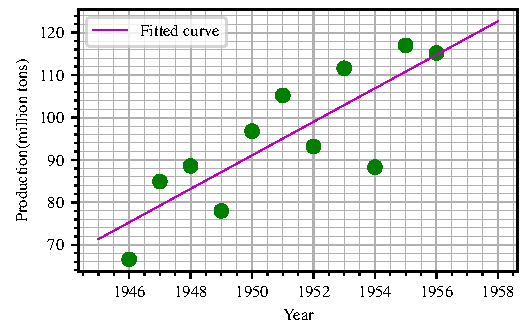
\includegraphics[scale=1.0,trim={0cm 0cm 0cm 0cm},clip]{./code/generatedPlots/fit_linear.pdf}
	\caption{Plot of original data along with fitted linear curve}
	\label{fig:fit_linear}
\end{figure}
%------------------Quadratic---------------------------%
\paragraph{(a) Quadratic curve fit:}For this the measurement matrix is:
\begin{align*}
H_{quadratic} = \begin{bmatrix}1 & t_0 & t_0^2\\ \vdots & \vdots & \vdots\\1 & t_{10} & t_{10}^2\end{bmatrix}.
\end{align*}
Our goal is to estimate $\beta = [\beta_0\ \beta_1\ \beta_2]^T$ such that the error,
\begin{align*}
e = y - H_{quadratic}\beta,
\end{align*}
is minimized in least square sense. Fig.~\ref{fig:fit_quadratic} shows the plot of original data along with the fitted least square curve.
\begin{figure}[h]
	\centering
	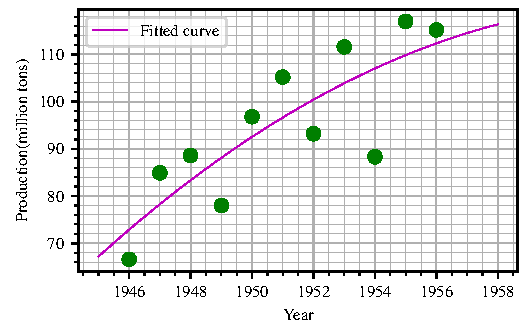
\includegraphics[scale=1.0,trim={0cm 0cm 0cm 0cm},clip]{./code/generatedPlots/fit_quadratic.pdf}
	\caption{Plot of original data along with fitted quadratic curve}
	\label{fig:fit_quadratic}
\end{figure}
%------------------Cubic---------------------------%
\paragraph{(a) Cubic curve fit:}For this the measurement matrix is:
\begin{align*}
H_{cubic} = \begin{bmatrix}1 & t_0 & t_0^2 & t_0^3\\ \vdots & \vdots & \vdots & \vdots\\1 & t_{10} & t_{10}^2 & t_{10}^3\end{bmatrix}.
\end{align*}
Our goal is to estimate $\beta = [\beta_0\ \beta_1\ \beta_2\ \beta_3]^T$ such that the error,
\begin{align*}
e = y - H_{cubic}\beta,
\end{align*}
is minimized in least square sense. Fig.~\ref{fig:fit_cubic} shows the plot of original data along with the fitted least square curve.
\begin{figure}[h]
	\centering
	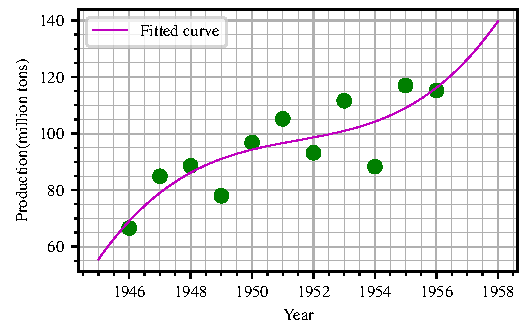
\includegraphics[scale=1.0,trim={0cm 0cm 0cm 0cm},clip]{./code/generatedPlots/fit_cubic.pdf}
	\caption{Plot of original data along with fitted cubic curve}
	\label{fig:fit_cubic}
\end{figure}
%------------------Quartic---------------------------%
\paragraph{(a) Quartic curve fit:}For this the measurement matrix is:
\begin{align*}
H_{quartic} = \begin{bmatrix}1 & t_0 & t_0^2 & t_0^3 & t_0^4\\ \vdots & \vdots & \vdots & \vdots & \vdots\\1 & t_{10} & t_{10}^2 & t_{10}^3 & t_{10}^4\end{bmatrix}.
\end{align*}
Our goal is to estimate $\beta = [\beta_0\ \beta_1\ \beta_2\ \beta_3\ \beta_4]^T$ such that the error,
\begin{align*}
e = y - H_{quartic}\beta,
\end{align*}
is minimized in least square sense. Fig.~\ref{fig:fit_quartic} shows the plot of original data along with the fitted least square curve.
\begin{figure}[h]
	\centering
	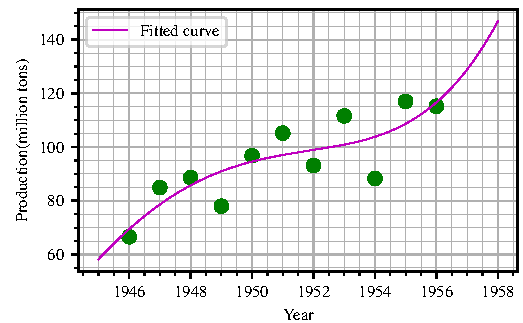
\includegraphics[scale=1.0,trim={0cm 0cm 0cm 0cm},clip]{./code/generatedPlots/fit_quartic.pdf}
	\caption{Plot of original data along with fitted quartic curve}
	\label{fig:fit_quartic}
\end{figure}
\newline
The following table shows the RMS errors and the prediction of steel production in 1957 for each of the polynomial curve fit:
\begin{center}
	\begin{tabular}{||c | c | c ||} 
		\hline
		Polynomial type & RMS error & Prediction of 1957 production (million tons)\\ [0.5ex] 
		\hline\hline
		Linear & $8.782$ & $118.715$\\
		\hline
		Quadratic & $8.666$ & $114.53$\\
		\hline
		Cubic & $8.289$ & $126.188$\\
		\hline
		Quartic & $8.282$ & $128.86$\\ [1ex]
		\hline
	\end{tabular}
\end{center}
 
    %----------------------------------------------------------------------------------------
%	SOLUTION 2
%----------------------------------------------------------------------------------------
\subsection*{Problem 2}
The dynamic system in this problem is given by,
\begin{align*}
	\dot{x} &= w\\
	\mathbb{E}[w] &= 0\\
	\mathbb{E}[w(t)w(\tau)] &= Q_c\delta(t-\tau)\\
	Q_c &= 1.
\end{align*}
%----------------------------------------------------------------------------------------
%	SOLUTION 2.a
%----------------------------------------------------------------------------------------
\paragraph{2.a} The dynamic system equation can be written as:
\begin{align*}
	\dot{x} &= 0x + 0u + w.
\end{align*}
Therefore, $A=0$ and $B=0$.
%----------------------------------------------------------------------------------------
%	SOLUTION 2.b
%----------------------------------------------------------------------------------------
\paragraph{2.b} $F$ and $G$ matrices of the discretized system can be derived as:
\begin{align*}
	F &= e^{AT}\\
	&= 1,
\end{align*}
where $T$ is the sampling interval equal to $1$ sec. Also,
\begin{align*}
	G &= e^{AT}\int_{0}^{T}e^{-A\alpha}\text{d}\alpha B\\
	&= 0.
\end{align*}
%----------------------------------------------------------------------------------------
%	SOLUTION 2.c
%----------------------------------------------------------------------------------------
\paragraph{2.c}The covariance of discrete process noise is:
\begin{align*}
	Q &= \int_{t_{k-1}}^{t_k}\int_{t_{k-1}}^{t_k}e^{A(t_k-\tau)}\mathbb{E}[w(\tau)w(\alpha)]e^{A^T(t_k-\alpha)}\text{d}\tau\text{d}\alpha\\
	&= \int_{t_{k-1}}^{t_k}\int_{t_{k-1}}^{t_k} Q_c \delta(\tau-\alpha)\text{d}\tau\text{d}\alpha\\
	&= \int_{t_{k-1}}^{t_k}Q_c\text{d}\tau\\
	&= Q_c(t_k-t_{k-1})\\
	&= Q_cT\\
	&= T\\
	&= 1.
\end{align*}
%----------------------------------------------------------------------------------------
%	SOLUTION 2.d
%----------------------------------------------------------------------------------------
\paragraph{2.d}The plot from the Monte-Carlo simulation is shown in Fig.~\ref{fig:q2_d}.
\begin{figure}[h]
	\centering
	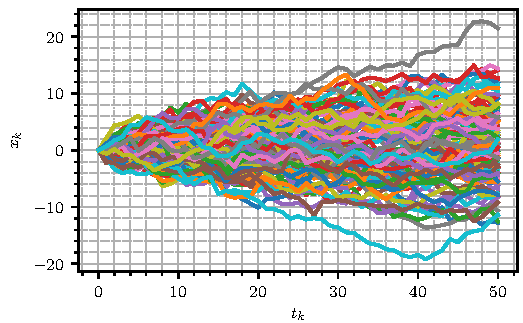
\includegraphics[scale=1.0,trim={0cm 0cm 0cm 0cm},clip]{./code/generatedPlots/q2_d.pdf}
	\caption{Q2.d: Monte-Carlo simulation of the dynamic process}
	\label{fig:q2_d}
\end{figure}
Ensemble standard deviation at $t_k=5,25$ and $50$ are $2.044, 4.99$ and $6.49$ respectively.
%----------------------------------------------------------------------------------------
%	SOLUTION 2.e
%----------------------------------------------------------------------------------------
\paragraph{2.e}The plot from the Monte-Carlo simulation is shown in Fig.~\ref{fig:q2_e}.
\begin{figure}[h]
	\centering
	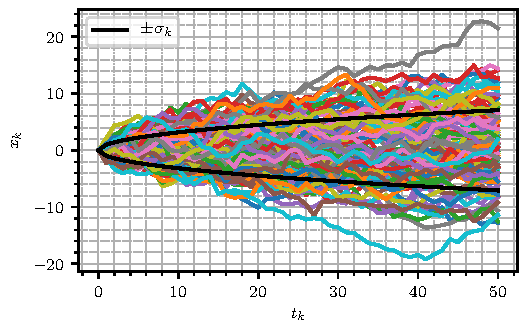
\includegraphics[scale=1.0,trim={0cm 0cm 0cm 0cm},clip]{./code/generatedPlots/q2_e.pdf}
	\caption{Q2.e: Monte-Carlo simulation along with plot from covariance analysis}
	\label{fig:q2_e}
\end{figure}
Values of $\sigma$ at $t_k=5$ and $10$ are $2.23$ and $3.16$ respectively.
%----------------------------------------------------------------------------------------
%	SOLUTION 2.f
%----------------------------------------------------------------------------------------
\paragraph{2.f}If I do not have any historical state measurements in hand, I would go for covariance analysis because it gives the theoretical state estimate standard deviation while to prove that Monte-Carlo simulation gives an accurate prediction of covariance, I need to run the simulation for many time, ideally infinite times. Usually, we go for Monte-Carlo where it is not possible to calculate the quantity theoretically. However, If I have historical state measurements in hand, I can check for any outliers or modeling error by doing Monte-Carlo analysis and compare that with the historical measurements.
\paragraph{Git location of the code:} The code file has been attached as a PDF file ('script\_q3.pdf'). Moreover, the code can be found at\\
\url{https://github.umn.edu/dey00011/EE5251\_optimal\_filter\_estimation/tree/master/HW3/code}
    %----------------------------------------------------------------------------------------
%	SOLUTION 3
%----------------------------------------------------------------------------------------
\subsection*{Problem 3}
$x$ is uniformly distributed on $[-1,1]$. Therefore, the PDF of $x$ is:
\begin{align*}
	f_X(x) = \begin{cases}
		\frac{1}{2},\ \text{ if } x \in [-1,1]\\
		0,\ \text{ otherwise }.
	\end{cases}
\end{align*}
Therefore, the expected value of $y=e^x$ is given by
\begin{align*}
	\bar{y} = E[y] &= \int_{-\infty}^{\infty} e^x f_X(x)\text{d}x\\
	&= \frac{1}{2}\int_{-1}^{1} e^x \text{d}x\\
	&= \frac{1}{2}\left[e-\frac{1}{e}\right]\\
	&= 1.175.
\end{align*}
The mean of $x$ is $\bar{x} = \frac{1}{2}(1-1) = 0$ and the covariance of $x$ is:
\begin{align*}
	P &= E[xx^T]\\
	&= E[x^2]\\
	&= \int_{-1}^{1} x^2 f_X(x)\text{d}x\\
	&= \frac{1}{2} \int_{-1}^{1} x^2\text{d}x\\
	&= \frac{1}{3}.
\end{align*}
First, we form two sigma points,
\begin{align*}
	x^{(1)} &= \sqrt{P} = \frac{1}{\sqrt{3}}\\
	x^{(2)} &= -\sqrt{P} = -\frac{1}{\sqrt{3}}.
\end{align*}
Then we calculate the non-linear transformation of the sigma points,
\begin{align*}
	y^{(1)} &= e^{x^{(1)}} = 1.781\\
	y^{(2)} &= e^{x^{(2)}} = 0.5614.
\end{align*}
Therefore, the approximated mean of $y$ is given by,
\begin{align*}
	\bar{y}_u &= \frac{1}{2}\sum_{i=1}^{2}y^{(i)}\\
	&= \frac{1}{2}[1.781+0.5614]\\
	&= 1.1712.
\end{align*}
    %----------------------------------------------------------------------------------------
%	SOLUTION 4
%----------------------------------------------------------------------------------------
\subsection*{Problem 4}
The dynamic model of the population system is:
\begin{align*}
	p_{k+1} &= 0.5p_k + 2f_k\\
	f_{k+1} &= f_k + w_f\\
	y_k &= p_k + v_k,
\end{align*}
where $w_f \sim \mathcal{N}(0, 10)$ and $v_k \sim \mathcal{N}(0,10)$. In matrix form,
\begin{align*}
	\begin{bmatrix}p_{k+1}\\f_{k+1}\end{bmatrix} &= \begin{bmatrix}0.5&2\\0&1\end{bmatrix}\begin{bmatrix}p_k\\f_k\end{bmatrix} + \begin{bmatrix}0\\w_k\end{bmatrix}\\
	y_k &= \begin{bmatrix}1&0\end{bmatrix}\begin{bmatrix}p_k\\f_k\end{bmatrix}+v_k.
\end{align*}
Therefore, in this problem $F = \begin{bmatrix}0.5&2\\0&1\end{bmatrix}$, $G=0$, $Q=\begin{bmatrix}0&0\\0&10\end{bmatrix}$, $R=10$ and $H = \begin{bmatrix}1&0\end{bmatrix}$.
%----------------------------------------------------------------------------------------
%	SOLUTION 4.a
%----------------------------------------------------------------------------------------
\paragraph{4.a} Fig.~\ref{fig:q4_population} shows the true and estimated population for $10$ time steps.
%%%%%%%%%%%%%%%%%%%%%%% POPULATION GRAPH %%%%%%%%%%%%%%%%%%%%%
\begin{figure}[!h]
	\centering
	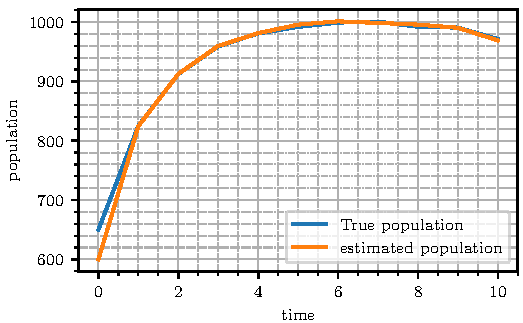
\includegraphics[scale=1.0,trim={0cm 0cm 0cm 0cm},clip]{./code/generatedPlots/q4_population.pdf}
	\caption{Q4.a: True and estimated population for 10 time steps}
	\label{fig:q4_population}
\end{figure}
Fig.~\ref{fig:q4_food} shows the true and estimated food supply for $10$ time steps.
%%%%%%%%%%%%%%%%%%%%%%% FOOD GRAPH %%%%%%%%%%%%%%%%%%%%%
\begin{figure}[!h]
	\centering
	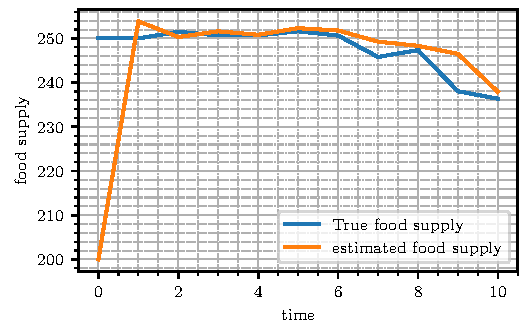
\includegraphics[scale=1.0,trim={0cm 0cm 0cm 0cm},clip]{./code/generatedPlots/q4_food.pdf}
	\caption{Q4.a: True and estimated food supply for 10 time steps}
	\label{fig:q4_food}
\end{figure}
Fig.~\ref{fig:q4_std_dev} shows the standard deviation (both $\pm$) of population and food supply estimates for $10$ time steps.
%%%%%%%%%%%%%%%%%%%%%%% STD DEV FOOD+POPULATION GRAPH %%%%%%%%%%%%%%%%%%%%%
\begin{figure}[!h]
	\centering
	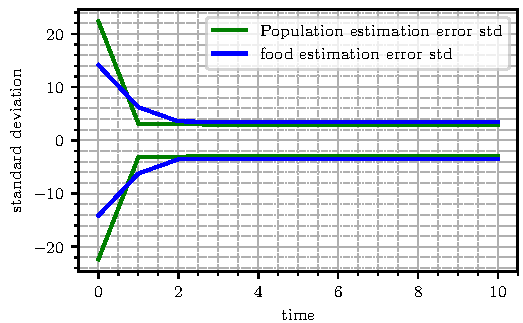
\includegraphics[scale=1.0,trim={0cm 0cm 0cm 0cm},clip]{./code/generatedPlots/q4_std_dev.pdf}
	\caption{Q4.a: Standard deviation of estimated population and food supply for 10 time steps}
	\label{fig:q4_std_dev}
\end{figure}
Fig.~\ref{fig:q4_kal_gain} shows the Kalman gains for population and food supply estimates for $10$ time steps.
%%%%%%%%%%%%%%%%%%%%%%% KALMAN GAINS GRAPH %%%%%%%%%%%%%%%%%%%%%
\begin{figure}[!h]
	\centering
	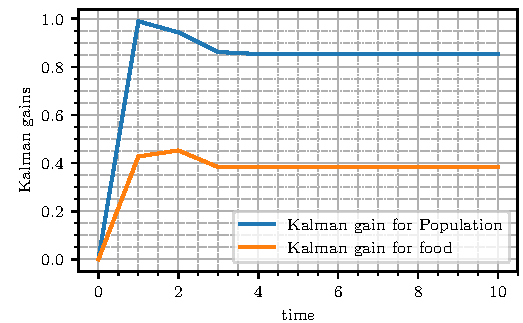
\includegraphics[scale=1.0,trim={0cm 0cm 0cm 0cm},clip]{./code/generatedPlots/q4_kal_gain.pdf}
	\caption{Q4.a: Kalman gains for population and food supply for 10 time steps}
	\label{fig:q4_kal_gain}
\end{figure}
%----------------------------------------------------------------------------------------
%	SOLUTION 4.b
%----------------------------------------------------------------------------------------
\paragraph{4.b}Fig.~\ref{fig:q4_std_dev_theoretical} shows the standard deviation (both $\pm$) of population and food supply estimates for $10$ time steps along with the steady state theoretical values (computed using covariance analysis).
%%%%%%%%%%%%%%%%%%%%%%% KALMAN GAINS GRAPH %%%%%%%%%%%%%%%%%%%%%
\begin{figure}[!h]
	\centering
	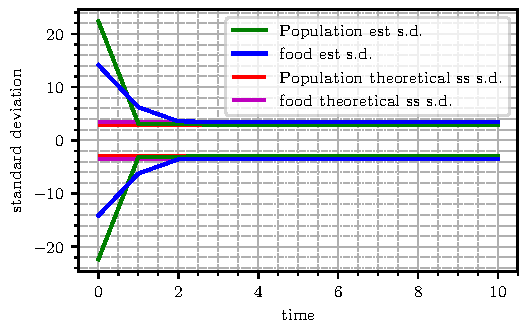
\includegraphics[scale=1.0,trim={0cm 0cm 0cm 0cm},clip]{./code/generatedPlots/q4_std_dev_theoretical.pdf}
	\caption{Q4.b: Standard deviations of population and food supply estimates for 10 time steps along with steady state(ss) theoretical values}
	\label{fig:q4_std_dev_theoretical}
\end{figure}
From Fig.~\ref{fig:q4_std_dev_theoretical}, we can see that the steady state theoretical values of standard deviations of the population and food supply estimates do not closely match with the estimated standard deviations of the same. This happens because $10$ time steps are not enough for the Kalman filter to converge closely to the theoretical value computed from covarinace analysis. We can see the improvement in 4.c.
%----------------------------------------------------------------------------------------
%	SOLUTION 4.c
%----------------------------------------------------------------------------------------
\paragraph{4.c}Fig.~\ref{fig:q4_std_dev_theoretical_1000} shows the standard deviation (both $\pm$) of population and food supply estimates for $1000$ time steps along with the steady state theoretical values (computed using covariance analysis).
%%%%%%%%%%%%%%%%%%%%%%% KALMAN GAINS GRAPH %%%%%%%%%%%%%%%%%%%%%
\begin{figure}[!h]
	\centering
	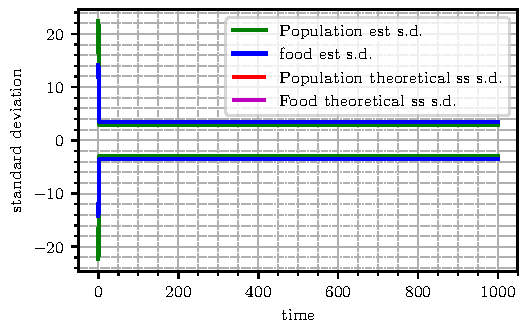
\includegraphics[scale=1.0,trim={0cm 0cm 0cm 0cm},clip]{./code/generatedPlots/q4_std_dev_theoretical_1000.pdf}
	\caption{Q4.c: Standard deviations of population and food supply estimates for 1000 time steps along with steady state(ss) theoretical values}
	\label{fig:q4_std_dev_theoretical_1000}
\end{figure}
From Fig.~\ref{fig:q4_std_dev_theoretical_1000}, we can see that the estimated standard deviations of the population and food supply converge to the steady state theoretical values as time goes by. Therefore, we can see that $1000$ time steps really improves the performance of the Kalman filter.
    %----------------------------------------------------------------------------------------
%	SOLUTION 5.a
%----------------------------------------------------------------------------------------
\subsection*{Problem 5.a}
The scalar system is given by
\begin{align*}
	x_{k+1} &= x_k + w_k,\ w_k \sim U[-1,1]\\
	y_k &= x_k + v_k,\ v_k \sim U[-1,1]\\
	x_0 &\sim U[-1,1].
\end{align*}
Therefore, the pdf of $x_1$ given $Y_0$ is 
\begin{align*}
	p(x_1|Y_0) &= \int_{-\infty}^{\infty}p(x_1|x_0)p(x_0|Y_0)\text{d}x_0\\
	&= \int_{-1}^{1}p(x_1|x_0)p(x_0)\text{d}x_0\hspace*{1cm}[\because x_0 \sim U[-1,1]]\\
	&= \frac{1}{2}\int_{-1}^{1}p(x_1|x_0)\text{d}x_0.
\end{align*}
Now,
\begin{align*}
	& x_1 = x_0+w_0\\
	\implies & w_0 = x_1-x_0.
\end{align*}
and,
\begin{align*}
	p(w_0) = p(x_1-x_0) = p(x_1|x_0) \sim U[-1,1] = \begin{cases}
		\frac{1}{2},\ \text{ if } -1 \leq x_1-x_0 \leq 1\\
		0,\ \text{ otherwise }.
	\end{cases}
\end{align*}
Therefore, if, $2 \geq x_1 \geq 0$, then
\begin{align*}
	p(x_1|Y_0) &= \frac{1}{2}\int_{-1+x_1}^{1}\frac{1}{2}\text{d}x_0\\
	&= \frac{1}{4}(2-x_1).
\end{align*}
If $-2 \leq x_1 <0$, then,
\begin{align*}
	p(x_1|Y_0) &= \frac{1}{2}\int_{-1}^{1+x_1}\frac{1}{2}\text{d}x_0\\
	&= \frac{1}{4}(x_1+2).
\end{align*}
Therefore,
\begin{align}\label{eq:q5_1}
	p(x_1|Y_0) = \begin{cases}
		\frac{1}{4}(2-x_1),\ \text{ if }0 \leq x_1 \leq 2\\
		\frac{1}{4}(x_1+2),\ \text{ if }-2 \leq x_1 < 0\\
		0, \text{ otherwise }.
	\end{cases}
\end{align}
Now,
\begin{align*}
	p(x_1|Y_1) &= \frac{p(y_1|x_1)p(x_1|Y_0)}{p(y_1|Y_0)}.
\end{align*}
Now,
\begin{align*}
	p(y_1|x_1) = p(v_1) = p(y_1-x_1) = \begin{cases}
		\frac{1}{2},\ \text{ if }-1\leq y_1-x_1\leq 1\\
		0, \text{ otherwise }.
	\end{cases}
\end{align*}
It is given that $y_1=1$. Therefore,
\begin{align*}
	p(y_1|x_1) = \begin{cases}
		\frac{1}{2},\ \text{ if }0\leq x_1 \leq 2\\
		0,\ \text{ otherwise }.
	\end{cases}
\end{align*}
Also,
\begin{align*}
	p(y_1|Y_0) &= \int_{-\infty}^{\infty}p(y_1|x_1)p(x_1|Y_0)\text{d}x_1\\
	&= \int_{0}^{2}\frac{1}{2}p(x_1|Y_0)\text{d}x_1\\
	&= \frac{1}{2}\int_{0}^{2}\frac{1}{4}(2-x_1)\text{d}x_1 \hspace*{1cm}[\text{ from }(\ref{eq:q5_1})]\\
	&= \frac{1}{8}[4-2] = \frac{1}{4}.
\end{align*}
Therefore,
\begin{align*}
	p(x_1|Y_1) &= \begin{cases}
		\frac{\frac{1}{2}\frac{1}{4}(2-x_1)}{\frac{1}{4}} = 1-\frac{x_1}{2},\ \text{ if }0\leq x_1 \leq 2\\
		0,\ \text{ otherwise }.
	\end{cases}
\end{align*}
%----------------------------------------------------------------------------------------
%	SOLUTION 5.b
%----------------------------------------------------------------------------------------
\subsection*{Problem 5.b}
In this problem, $Q_k=E[w_kw_k^T] = \frac{1}{3}$ and $R_k = E[v_kv_k^T] = \frac{1}{3}$. Also $F=H=1$.
\newline
We can find the Kalman filter estimate of $\hat{x}_1^{+}$ in the following way:
\begin{align*}
	\hat{x}_0^{+} &= E[x_0] = 0 \hspace{1cm}[\because x_0 \sim U[-1,1]]\\
	P_0^{+} &= E[x_0^2] = \frac{1}{3}\\
	P_1^- &= FP_0^+F^T + Q = \frac{1}{3}+\frac{1}{3} = \frac{2}{3}\\
	K_1 &= P_1^-H^T(HP_1^-H^T+R)^{-1} = \frac{2}{3}\\
	\hat{x}_1^- &= F\hat{x}_0^+ = 0\\
	\hat{x}_1^+ &= \hat{x}_1^-+K_1(y_1-H\hat{x}_1^-) = 0+\frac{2}{3}(1-0) = \frac{2}{3}.
\end{align*}
Kalman filter estimate of $\hat{x}^+$ is indicative of MAP estimate of the pdf of $p(x_1|Y_1)$. We can calculate it theoretically and find that it is close enough to the Kalman filter estimate.


    %\input{problem_2}
    %\input{solution_2}
\end{document}